\documentclass[a4paper]{article}

% Basic packages
\usepackage{fontspec}
\XeTeXlinebreaklocale "zh"    % 启用中文断行（XeTeX 内建，无需 xeCJK）
\XeTeXlinebreakskip = 0pt plus 1pt
\setmainfont{Songti SC}
\setsansfont{Heiti SC}
\setmonofont{Menlo}
\usepackage{amsmath, amssymb}
\usepackage{graphicx}
\usepackage[margin=2.5cm]{geometry}
\usepackage[most]{tcolorbox}
\usepackage{etoolbox}
\usepackage{listings}
\usepackage{hyperref}
\usepackage{booktabs}
\usepackage{subcaption}
\usepackage{float}

% Chinese font setup (macOS system fonts, no ctex needed)
\setmainfont{Songti SC}
\setsansfont{Heiti SC}
\setmonofont{Menlo}
\newcommand{\song}{\fontspec{Songti SC}}
\newcommand{\hei}{\fontspec{Heiti SC}}
\newcommand{\kai}{\fontspec{KaiTi}}
\newcommand{\fangsong}{\fontspec{FangSong}}

% ===== Highlight boxes =====
\newtcolorbox{knowledgebox}[1]{
    enhanced, colback=blue!5!white, colframe=blue!75!black, colbacktitle=blue!75!black,
    coltitle=white, fonttitle=\bfseries, title=#1, attach boxed title to top left={yshift=-2mm, xshift=2mm},
    boxrule=1pt, sharp corners
}

\newtcolorbox{importantbox}[1]{
    enhanced, colback=yellow!10!white, colframe=yellow!80!black, colbacktitle=yellow!80!black,
    coltitle=black, fonttitle=\bfseries, title=#1, sharp corners
}

\newtcolorbox{warningbox}[1]{
    enhanced, colback=red!5!white, colframe=red!75!black, colbacktitle=red!75!black,
    coltitle=white, fonttitle=\bfseries, title=#1, sharp corners
}

\newtcolorbox{practicebox}[1]{
    enhanced, colback=green!5!white, colframe=green!60!black, colbacktitle=green!60!black,
    coltitle=white, fonttitle=\bfseries, title=#1, sharp corners
}

% ===== Code listings =====
\lstset{
    basicstyle=\ttfamily\small,
    keywordstyle=\color{blue},
    stringstyle=\color{red!60!black},
    commentstyle=\color{green!60!black},
    breaklines=true,
    frame=single,
    numbers=left,
    numberstyle=\tiny\color{gray},
    captionpos=b,
    extendedchars=false
}

% ===== Front-page metadata =====
\newcommand{\notetitle}{CS336 Lecture 14：数据（下）——过滤与去重}
\newcommand{\notesubtitle}{Stanford CS336: Language Modeling from Scratch (Spring 2025)}
\newcommand{\noteauthors}{讲师：Tatsu Hashimoto \quad 笔记：ZCode}
\newcommand{\notedate}{2026-07-14}
\newcommand{\videochannel}{Stanford CS336}
\newcommand{\videopublishdate}{2025 Spring}
\newcommand{\videoduration}{79 分钟}
\newcommand{\videourl}{https://www.youtube.com/watch?v=SQ3fZ1sAqXI}
\newcommand{\videocoverpath}{cover.jpg}

\begin{document}

% ===== Title page =====
\begin{titlepage}
\centering
{\Large 课程笔记\par}
\vspace{1.2cm}
{\huge\bfseries \notetitle\par}
\vspace{0.3cm}
{\large \notesubtitle\par}
\vspace{0.5cm}
{\large \noteauthors\par}
\vspace{0.3cm}
{\large \notedate\par}
\vspace{1.0cm}

\includegraphics[width=0.82\textwidth,height=0.40\textheight,keepaspectratio]{\videocoverpath}\par

\vfill
\begin{tcolorbox}[width=0.9\textwidth, colback=black!2!white, colframe=black!60, sharp corners]
\textbf{视频作者/频道}：\videochannel\par
\textbf{发布日期}：\videopublishdate\par
\textbf{视频时长}：\videoduration\par
\textbf{视频链接}：\href{\videourl}{\nolinkurl{\videourl}}
\end{tcolorbox}
\end{titlepage}

\tableofcontents
\newpage

%% --- 正文内容开始 ---

\section{导论：为什么数据（下）是一门算法课}

这是关于数据的第二讲。上一讲回顾了从 BERT 到 Llama 再到 Homo 等一系列语言模型所用数据集的历史脉络，并强调了一个核心观点：\textbf{数据不会从天上掉下来}。它们往往存在于各种在线服务中，必须显式地爬取或导出，然后经过大量处理。这些处理步骤包括把原始 HTML 转成纯文本，再做语言识别、质量过滤、毒性过滤、去重等等。

\begin{figure}[H]
\centering
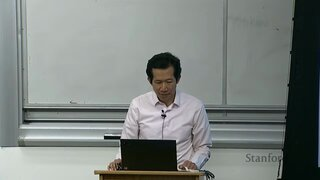
\includegraphics[width=0.92\textwidth]{figures/01_title.jpg}
\caption{Lecture 14：Data 2，聚焦过滤与去重的算法细节\protect\footnotemark}
\end{figure}
\footnotetext{视频画面时间区间：00:00:05--00:00:30。}

本讲将深入两件"机械学"层面的事情：一是\textbf{质量过滤（quality filtering）}是如何工作的，二是\textbf{去重（deduplication）}是如何工作的。与上一讲偏综述不同，本讲会大量涉及经典的大数据处理算法，对喜欢数学的同学会相当友好。

\begin{knowledgebox}{本讲三大主线}
\begin{enumerate}
    \item \textbf{过滤算法}：n-gram 模型、线性分类器（FastText）、重要性重采样（importance resampling）。
    \item \textbf{过滤的应用}：同一套"过滤机器"可用于语言识别、质量过滤、毒性过滤等。
    \item \textbf{去重算法}：精确去重（哈希表、Bloom Filter）与近似去重（MinHash + LSH）。
\end{enumerate}
\end{knowledgebox}

\section{过滤：从原始数据中找出"像目标"的子集}

\subsection{过滤的统一抽象}

所有过滤任务都可以抽象成下面这个图景：

\begin{figure}[H]
\centering
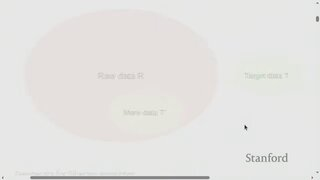
\includegraphics[width=0.92\textwidth]{figures/02_filtering_primitive.jpg}
\caption{过滤原语：给定少量高质量目标数据 $T$ 与海量原始数据 $R$，找出与 $T$ 相似的子集 $T'$\protect\footnotemark}
\end{figure}
\footnotetext{视频画面时间区间：00:01:30--00:02:10。}

你拥有一份\textbf{目标数据（target data）} $T$：它数量很少但质量很高（比如维基百科、教科书）。你还有一份\textbf{原始数据（raw data）} $R$：它体量巨大（比如 Common Crawl 的整个网页）。目标是找到一个子集 $T' \subseteq R$，使得 $T'$ 与 $T$ 在分布上相似。

\begin{importantbox}{过滤算法必须满足的两个性质}
\begin{enumerate}
    \item \textbf{泛化能力}：$T'$ 不能只是 $T$ 的复制——你已经有 $T$ 了，复制没有意义。它必须从 $R$ 中"发现"新的、与 $T$ 同分布的数据。
    \item \textbf{极快的速度}：算法要能在整个互联网规模的数据上运行。如果用一个巨大的模型去打分，它的开销可能与训练本身相当，那就得不偿失了。
\end{enumerate}
\end{importantbox}

本讲会介绍三种实现这个抽象原语的具体方法。

\subsection{方法一：N-gram 语言模型（KenLM）}

第一种也是最经典的方法：在目标数据 $T$ 上训练一个 n-gram 语言模型，然后用它给 $R$ 中每个文档打分（计算困惑度），保留低困惑度（即高概率）的文档。

\begin{figure}[H]
\centering
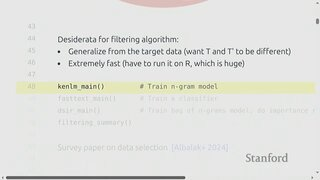
\includegraphics[width=0.92\textwidth]{figures/03_ngram_kenlm.jpg}
\caption{N-gram 语言模型：起点是最大似然估计，关键难点是稀疏计数\protect\footnotemark}
\end{figure}
\footnotetext{视频画面时间区间：00:02:30--00:03:30。}

起点是语言模型的\textbf{最大似然估计}。给定语料，估计条件概率：

\[
p(w_n \mid w_1, w_2, \dots, w_{n-1}) = \frac{\mathrm{count}(w_1, \dots, w_n)}{\mathrm{count}(w_1, \dots, w_{n-1})}
\]

也就是统计 n-gram 出现的次数，再除以（n-1)-gram 上下文出现的次数。原理非常简单。但实现高效的统计要费一番功夫，更关键的问题是\textbf{稀疏计数}：当 $n$ 增大时，大量合理的 n-gram 在语料中出现次数为零，这正是 n-gram 模型无法规模化、被维度诅咒困住的根因。

\begin{knowledgebox}{Kneser-Ney 平滑}
为了缓解零计数问题，Kneser-Ney 平滑提出：当高阶 n-gram 的证据不足时，就"回退（backoff）"到低阶 n-gram——把上下文去掉一个词，用 $(n-1)$-gram 来插值或回退。工业界常用一个开源实现 \texttt{KenLM}（最初为机器翻译开发），它实现了 Kneser-Ney 平滑。N-gram 建模的好处是非常简单——"拟合模型"本质上就是数 n-gram 然后归一化。
\end{knowledgebox}

\subsubsection*{KenLM 实战：困惑度演示}

讲师下载了一个在维基百科上训练好的 KenLM 模型，并给若干句子计算困惑度（perplexity）。

\begin{figure}[H]
\centering
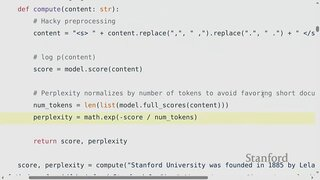
\includegraphics[width=0.92\textwidth]{figures/04_kenlm_demo.jpg}
\caption{KenLM 困惑度演示：维基百科句子得低困惑度，乱码得高困惑度\protect\footnotemark}
\end{figure}
\footnotetext{视频画面时间区间：00:05:50--00:06:50。}

\begin{itemize}
    \item "Stanford University was founded in 1885."（维基百科原句）$\to$ 困惑度约 87，合理。
    \item "this is taken from the CS336 website..."（同样是规范英语）$\to$ 困惑度略高，但仍合理，因为这种表达未必出现在维基百科。
    \item "ESDF" 这类纯乱码 $\to$ 高困惑度，符合预期。
    \item 某些"看起来不该"的句子被赋予低困惑度——n-gram 模型并不聪明，但做数据过滤\textbf{不需要}最聪明的模型，只要足够粗糙、足够快即可。
\end{itemize}

\begin{practicebox}{CCNet：首版 Llama 的数据管线}
Meta（当时还叫 Facebook）的 CCNet 论文，正是用 KenLM 实操这套流程：以\textbf{段落}为单位，按困惑度升序排序，仅保留 top $1/3$ 的段落。这就是首版 Llama 训练数据集的构建方式。这是个相当启发式（heuristic）的方法，但若你必须快速写出一个过滤管线，它确实"有点道理"。
\end{practicebox}

\begin{figure}[H]
\centering
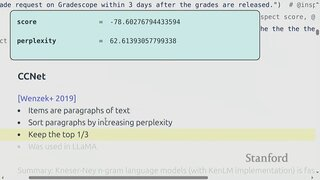
\includegraphics[width=0.92\textwidth]{figures/05_ccnet.jpg}
\caption{CCNet：按段落困惑度升序排序，保留前 1/3\protect\footnotemark}
\end{figure}
\footnotetext{视频画面时间区间：00:07:45--00:08:15。}

N-gram 建模的优点是\textbf{快}，缺点是\textbf{粗糙}。它只能看局部上下文，容易被对抗性构造的例子欺骗（把词序打乱它仍可能打高分），但作为"过滤掉纯垃圾网页"的工具已经够用。

\subsection{方法二：FastText 线性分类器}

第二种方法在实际中更流行，这就是 \textbf{FastText}。它同样出自 Meta，原本是为文本分类设计的。在 2016 年，许多人在搞复杂的神经网络分类器，FastText 论文则证明：一个几乎就是线性分类器的方法，效果不逊于那些花哨模型，却快得多。

\begin{figure}[H]
\centering
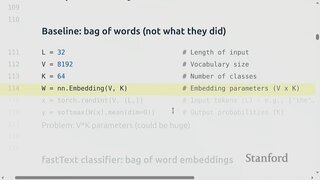
\includegraphics[width=0.92\textwidth]{figures/06_fasttext_arch.jpg}
\caption{FastText 动机：词袋线性分类的参数量爆炸，用隐层维度压缩\protect\footnotemark}
\end{figure}
\footnotetext{视频画面时间区间：00:09:30--00:10:30。}

动机如下：做词袋（bag-of-words）分类时，输入是长度为 $L$ 的句子，词表大小为 $V$，要分到 $K$ 个类别，立即需要一个 $V \times K$ 的矩阵。当 $V$、$K$ 都很大时，参数量爆炸，还会遇到稀疏问题。

\begin{importantbox}{FastText 的核心招式：维度压缩}
FastText 的做法是先做一次线性的"降维"：把词表空间 $V$ 映射到一个较小的隐层维度 $h$（可能小于 16），再从 $h$ 做分类。注意前向传播中\textbf{没有任何非线性}，它就是一个线性分类器（也可以看作矩阵分解）。参数量被大幅缩减，实现做了并行化和异步 SGD，因此非常快。
\end{importantbox}

\subsubsection*{哈希技巧（Hashing Trick）：处理 n-gram}

词袋丢失了词序信息，我们自然想用 n-gram。但 n-gram 的数量会爆炸式增长且理论上无界（回忆分词那一讲）。FastText 用一个非常简单的办法处理：\textbf{哈希}。

\begin{figure}[H]
\centering
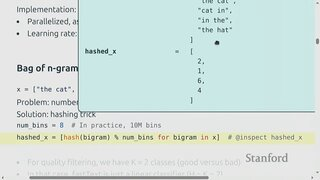
\includegraphics[width=0.92\textwidth]{figures/07_fasttext_hashing.jpg}
\caption{FastText 哈希技巧：把每个 n-gram 哈希到固定数量的桶里\protect\footnotemark}
\end{figure}
\footnotetext{视频画面时间区间：00:11:30--00:12:30。}

定义若干个桶（比如一千万个，示例里是 8 个），然后把每个 n-gram 哈希到某个桶。"the cat" 映射到 2，"cat in" 映射到 1，以此类推。当然会有\textbf{哈希冲突}，但我们接受它：优化损失时冲突会被自动"平均"掉——两个无关的词若哈希到同一桶，那个权重会近似代表它们的平均。

\begin{knowledgebox}{二分类视角}
数据过滤里常常把 FastText 当作 $K=2$ 的二分类器用：这个文档"好"还是"坏"？此时它就是一个普通的二元线性分类。
\end{knowledgebox}

当然，有了线性分类就能想到用 BERT 甚至 Llama 这样的"大模型"打分。唯一的问题是它们更慢。Web 数据太大，若把过滤模型做得太重，那部分算力还不如直接去训模型——你正打算把整个 web 过滤到 $1\%$，意味着分类器每次前向传播的开销必须远小于训练一遍数据的开销。

\subsection{方法三：重要性重采样（Importance Resampling）}

第三种方法更"有原则"（principled）：\textbf{Data Selection for Language Models using Importance Resampling}（DSIR）。思路是你有一个目标数据集 $D_P$（小）和一个原始数据集 $D_Q$（大），你构造一个\textbf{重要性权重估计器}——它是 n-gram 模型或 FastText 的"概率比"对应物，然后用它来抽样文档。

\begin{figure}[H]
\centering
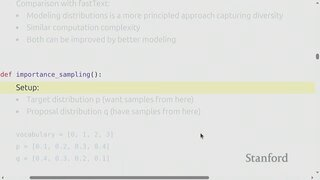
\includegraphics[width=0.92\textwidth]{figures/08_importance_resample.jpg}
\caption{重要性重采样基础：从提议分布 $Q$ 采样，用 $P/Q$ 重加权再重采样\protect\footnotemark}
\end{figure}
\footnotetext{视频画面时间区间：00:14:00--00:15:40。}

先复习一下重要性重采样的基本思想（它出现在粒子滤波、蒙特卡洛方法等很多场景）。你有一个\textbf{目标分布} $P$（你想从中采样），但只能从\textbf{提议分布} $Q$ 中采样。做法是：

\begin{enumerate}
    \item 从 $Q$ 采一堆样本（$Q$ 在某些位置概率更大，所以这些位置样本多）。
    \item 对每个样本计算权重 $w_i = P(x_i) / Q(x_i)$，归一化得到样本上的分布。
    \item 按这个分布\textbf{重采样}，从而平衡掉 $Q$ 的偏置——结果是样本更接近 $P$。
\end{enumerate}

\begin{warningbox}{$D_P$ 太小怎么办？}
回到数据选择：我们有的是数据集 $D_P$ 和 $D_Q$，不是分布。理论上可以分别拟合分布 $p$（给 $D_P$）和 $q$（给 $D_Q$），然后做重要性重采样。问题是 $D_P$ 非常小（高质量数据本就稀缺，这正是你想获得更多它的原因），小到不足以训练一个好的 $p$ 模型。
\end{warningbox}

解决办法还是\textbf{哈希 n-gram}。这里只用 unigram：把 $D_P$ 中每个 unigram 哈希到某个桶，统计每个桶的频次，估计每个哈希 unigram 的概率。

\begin{figure}[H]
\centering
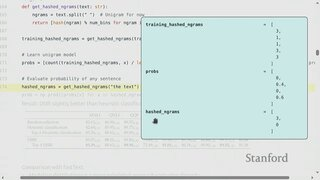
\includegraphics[width=0.92\textwidth]{figures/09_dsir_hashing.jpg}
\caption{DSIR：用哈希 unigram 估计目标分布 $p$ 与原始分布 $q$\protect\footnotemark}
\end{figure}
\footnotetext{视频画面时间区间：00:17:40--00:18:30。}

要评估一段新文本的概率，就把它的每个 unigram 哈希、再把对应概率相乘。可能不幸地遇到某个 unigram 概率为零（被清零），可以加一点平滑。注意 Python 的 \texttt{hash} 是非确定性的，每次运行结果都不同。

\begin{practicebox}{DSIR 的实验结果}
论文显示，相比 FastText 这种"启发式分类"的方法，DSIR 在 GLUE 上用 BERT 风格模型做评测，确实带来了一些提升（虽然增益并非巨大）。其核心思想在于：\textbf{建模整个分布}比二分类"在不在分布里"更有原则——你想匹配分布，而不是粗暴地分类。它同样快，也都可以通过增大 $n$ 或换用神经网络来改进打分模型。
\end{practicebox}

\subsection{三种方法的统一视角}

\begin{figure}[H]
\centering
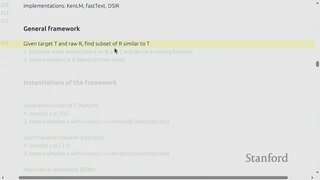
\includegraphics[width=0.95\textwidth]{figures/10_filtering_summary.jpg}
\caption{三种过滤方法的统一框架：拟合一个打分函数，再按打分保留高分的样本\protect\footnotemark}
\end{figure}
\footnotetext{视频画面时间区间：00:19:30--00:20:30。}

无论哪种方法，核心配方都是一样的：

\begin{importantbox}{过滤的统一配方}
\textbf{输入}：目标数据 $T$、原始数据 $R$。\par
\textbf{步骤}：基于 $T$（和可能的 $R$）估计一个打分函数 $s(\cdot)$，然后保留 $R$ 中 $s$ 高于某阈值的样本。
\begin{itemize}
    \item \textbf{KenLM}：$s(x) = p_T(x)$（或在目标上估计的困惑度），$R$ 不参与训练，保留 $s(x) > \tau$。可在阈值附近做一点随机化。
    \item \textbf{判别分类器（FastText）}：$s(x) = \Pr[x \text{ 来自 } T \text{ 而非 } R]$，保留 $s(x) > \tau$。
    \item \textbf{重要性重采样}：$s(x) = p(x) / q(x)$（两个生成模型之比，可以是 n-gram），按 $s$ 成比例地重采样。
\end{itemize}
\end{importantbox}

高层来看，它们都在做同一件事：拟合一个告诉你"什么像目标、而非原始"的分布，再把它套到原始数据上。

\subsection{课堂问答：n-gram 的局限}

有同学提问：n-gram 只看局部上下文，把词序打乱它仍打高分，这怎么保证文档质量？讲师承认这种对抗性欺骗的风险确实存在（演示里就有反例），但"平均而言"它还是管用的——只要一份文档看起来语法通顺、像新闻或科学论文，让模型给它高概率就够了。即使混入一些坏例子，也不是世界末日。\textbf{更准确地说，这些分类器主要是用来"过滤掉纯垃圾网页"的}。随着后面讲各种应用案例，这一点会越来越清楚。

\section{过滤的应用：同一台机器，多种用法}

同一套数据过滤机器，可以用于完全不同的任务。下面看三个典型应用：语言识别、质量过滤、毒性过滤。

\subsection{语言识别（Language Identification）}

语言识别的目标是从原始数据里找出特定语言的文本（比如英语、日语）。有人会问：为什么不直接在所有语言上训练？

\begin{figure}[H]
\centering
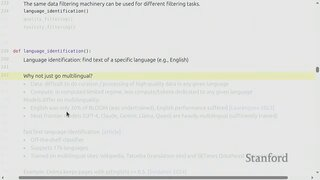
\includegraphics[width=0.92\textwidth]{figures/11_langid.jpg}
\caption{语言识别：FastText 提供开箱即用的多语言分类器\protect\footnotemark}
\end{figure}
\footnotetext{视频画面时间区间：00:24:00--00:25:00。}

\begin{warningbox}{多语言的两难}
\begin{itemize}
    \item 在给定语言上做高质量数据的策展和处理常常很困难。
    \item 如果训练数据混杂了所有语言，你在任何单一语言上花掉的算力和 token 都会变少，可能损害该语言的性能。比如 Bloom（约 2022 年）只有 30\% 是英语，导致其英语性能不如人意（其他语言则很强）。
    \item 当然，如果模型容量足够大，多语言之间甚至会产生\textbf{正向迁移}，所以前沿模型往往在一百多种语言上训练。
\end{itemize}
\end{warningbox}

最简单的做法是用 \texttt{FastText} 提供的开箱即用语言识别模型（它在维基百科、多语言翻译站点，以及"某些南欧新闻"上训练）。Dolma 数据集就是用它跑分类、保留英语概率 $> 0.5$ 的页面。

讲师现场测试了几个句子：标准的 "the quick brown fox..." 得到 English 标签但概率只有 71\%（比想象低）；重复句子不会让概率变化（说两遍同样的内容不会"更英语"）；德语、法语、意大利语的 \texttt{bonjour} 都被正确识别；但\textbf{代码}被分到了俄语、\textbf{数学}被很弱地分到英语——短句、低资源语言、英语方言、相近语言、语码转换（code switching）都是容易出错的场景。

\begin{knowledgebox}{教训}
"能下载、大家都在用"的分类器并不代表它总 work。务必亲自拿自己的数据跑一跑、看看它的失败模式。
\end{knowledgebox}

\subsection{案例研究：OpenWebMath}

\textbf{OpenWebMath}（约两年前的论文）是一个绝佳案例：把"数学"当成一门语言，去策展大规模数学文本语料。

\begin{figure}[H]
\centering
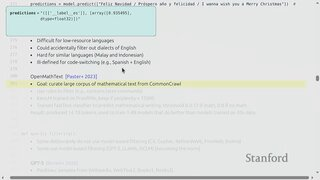
\includegraphics[width=0.92\textwidth]{figures/12_openwebmath.jpg}
\caption{OpenWebMath：规则过滤 + KenLM（在 Proofpile 上训练）+ FastText 三级流水线\protect\footnotemark}
\end{figure}
\footnotetext{视频画面时间区间：00:29:00--00:30:20。}

它的流水线是多级的：先用一些规则初筛；再在一个大规模证明语料库 \textbf{Proof pile} 上训练 KenLM，保留困惑度低于阈值的文档；同时还训练了一个 FastText 分类器来判定"是否是数学写作"。这里有个\textbf{取巧的阈值策略}：若规则已判定为数学，则 FastText 阈值放宽；若规则未判定为数学，则 FastText 阈值收紧。最终产出 150 亿 token，在其上训练的模型比在 20 倍数据量、未特化的模型上表现更好。

\begin{importantbox}{数据过滤的价值}
这正是数据过滤的典范用法：你本可以训练所有数据，但若你关心某个领域（如数学），就主动去获取更多该领域数据，瞄准那个目标数据集——这样训练会\textbf{高效得多}。
\end{importantbox}

\subsection{质量过滤（Quality Filtering）}

质量是个"什么算高质量"的笼统概念。早期一些论文明确不使用基于模型的质量过滤，但更近期的论文基本都"缴械投降"了——因为它确实让效果好得多。下面三个例子展示了质量过滤的三种哲学。

\begin{figure}[H]
\centering
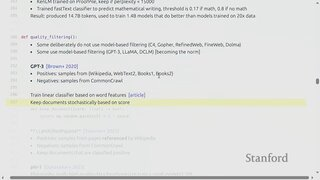
\includegraphics[width=0.95\textwidth]{figures/13_quality_filter.jpg}
\caption{质量过滤三例：GPT-3、Llama、Phi-1 的正负样本来源\protect\footnotemark}
\end{figure}
\footnotetext{视频画面时间区间：00:31:00--00:32:30。}

\begin{tabular}{p{2.2cm}p{4.5cm}p{4.5cm}p{2.8cm}}
\toprule
\textbf{论文} & \textbf{正样本来源} & \textbf{负样本来源} & \textbf{保留策略} \\
\midrule
GPT-3 & 非 Common Crawl 的高质量源 & Common Crawl 采样 & 训练线性分类器，按分数随机保留 \\
首版 Llama & 被\textbf{维基百科引用}的页面（不是维基本身） & Common Crawl 采样 & 分类为正即保留（无采样） \\
Phi-1 & GPT-4 标注的 10 万 Python 文档（教育价值评分） & --- & 随机森林 + codegen 嵌入 \\
\bottomrule
\end{tabular}

\vspace{0.3cm}

Phi-1 的哲学最为有趣：他们想要"像教科书一样"的高质量数据来训练一个很小的模型。

\begin{figure}[H]
\centering
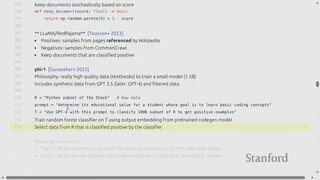
\includegraphics[width=0.92\textwidth]{figures/14_phi1.jpg}
\caption{Phi-1：用 GPT-4 判定教育价值，蒸馏成随机森林分类器\protect\footnotemark}
\end{figure}
\footnotetext{视频画面时间区间：00:33:30--00:34:20。}

他们的做法是：取 The Stack 的 Python 子集（The Stack 是从 GitHub 预处理的代码数据集），定义一个 prompt，让 \textbf{GPT-4} 判定每个文档"对一个想学基础编程概念的学生"的\textbf{教育价值}。用这个 prompt 标注 10 万份文档作为正例，训练一个\textbf{随机森林}分类器（输入特征是某个预训练 codegen 模型的嵌入），然后在整个 $R$ 上跑这个分类器筛数据。

\begin{practicebox}{$T$ 从哪来？——大模型生成 $T$ 的新范式}
Phi-1 最有意思的地方：\textbf{$T$ 并不预先存在}，它来自 prompt 一个强大的语言模型。随着模型越来越好，这种模式会越来越常见——你不必再去找"哪本书是高质量"的源，而是直接问模型："我要更多化学数据""我要更多做证明的数学数据"，让模型帮你产出 $T$，然后再套上前面那套配方。
\end{practicebox}

\begin{knowledgebox}{Phi-1 的结果}
基线（直接用 The Stack 的 Python 子集作为 $R$）：训练 9.6 万步后，HumanEval 只有 12\%。\par
Phi-1（同样架构、换成精筛后的数据）：仅 3.6 万步就达到 17\%。—\,成功。
\end{knowledgebox}

\subsection{毒性过滤（Toxicity Filtering）}

以 Dolma 论文为例讲毒性过滤。它用了一个数据集叫 \textbf{Jigsaw Toxic Comments}——源于一个旨在帮助人们在网上更好讨论的项目。他们在维基百科的 talk 页面上抓评论，让标注者标注：toxic / severe toxic / obscene / threat / insult / identity hate 等标签。Dolma 团队训练了\textbf{两个 FastText 分类器}，一个对应 hate，一个对应 NSFW。

\begin{figure}[H]
\centering
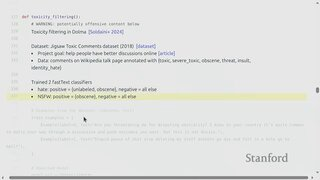
\includegraphics[width=0.92\textwidth]{figures/15_toxicity_jigsaw.jpg}
\caption{毒性过滤：Jigsaw 数据集 + 两个 FastText 二分类器\protect\footnotemark}
\end{figure}
\footnotetext{视频画面时间区间：00:36:00--00:37:00。}

讲师下载模型测试：第一句"are you threatening me for dispute neutrality"被判定 safe for work（看起来没问题）；第二句被标记为 NSFW。这些句子本身都算正常，可见分类器并非完美，但能给你一个直觉。

\section{去重：避免在海量副本上浪费算力}

讲完过滤，进入第二大块——\textbf{去重（deduplication）}。

\subsection{为什么需要去重：两类重复}

网页天然就有大量重复内容，分两类：

\begin{figure}[H]
\centering
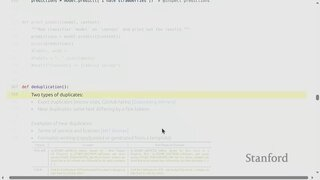
\includegraphics[width=0.92\textwidth]{figures/16_dedup_intro.jpg}
\caption{两类重复：精确重复（镜像）与近似重复（改了几个 token）\protect\footnotemark}
\end{figure}
\footnotetext{视频画面时间区间：00:37:00--00:38:00。}

\begin{enumerate}
    \item \textbf{精确重复（exact duplicates）}：源于镜像（mirroring）。比如 Project Gutenberg 的同一个站点被镜像到许多 URL，Common Crawl 爬下来并不知道它们是镜像，就会给出完全相同的内容。
    \item \textbf{近似重复（near duplicates）}：基本相同、只差几个 token。例如 MIT 许可证在全网被复制了无数次；有人复制时漏掉一个逗号；或者模板系统生成的内容（把"Canada"换成"USA"和另一个航班）。
\end{enumerate}

\begin{figure}[H]
\centering
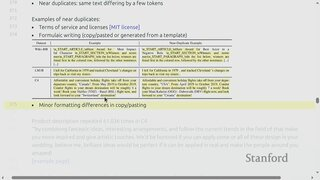
\includegraphics[width=0.95\textwidth]{figures/17_near_dup_examples.jpg}
\caption{近似重复实例：改写、漏逗号、模板填实体\protect\footnotemark}
\end{figure}
\footnotetext{视频画面时间区间：00:39:00--00:40:00。}

\subsubsection*{极端案例：C4 中重复 6.1 万次的句子}

\begin{figure}[H]
\centering
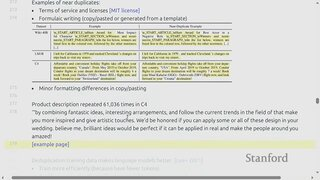
\includegraphics[width=0.92\textwidth]{figures/18_c4_61k.jpg}
\caption{C4 中某条英语句子被重复了 6.1 万次（来源于亚马逊某产品页）\protect\footnotemark}
\end{figure}
\footnotetext{视频画面时间区间：00:40:30--00:41:00。}

在 C4（用一组"是否像英语"的规则筛过）里，有一条英语句子竟然重复了\textbf{61,000 次}。追根溯源，它来自亚马逊上一个有涂鸦画的产品页。这段文本本身\textbf{并不坏}——是完好的英语——但你绝对不想对它做 61,000 个 epoch。

\begin{importantbox}{去重 vs. 质量过滤}
质量过滤说："这段数据我不想再训练。"去重说："它本身没问题，但我只想要少数几份，而不是 61,000 份。" 两者是\textbf{互补}的。
\end{importantbox}

\subsection{去重的收益}

\begin{figure}[H]
\centering
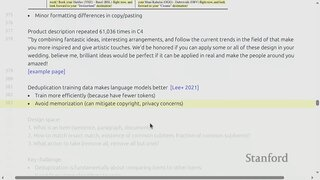
\includegraphics[width=0.92\textwidth]{figures/19_dedup_benefits.jpg}
\caption{去重的两大收益：训练效率 + 避免记忆\protect\footnotemark}
\end{figure}
\footnotetext{视频画面时间区间：00:41:15--00:42:00。}

已有研究证明去重能让语言模型更好：

\begin{enumerate}
    \item \textbf{训练更高效}：去重减少了 token 数。如果没有丢失信息，就能省下大量算力。
    \item \textbf{避免记忆（memorization）}：语言模型会记住训练数据，这对版权和隐私不利（会原样复述训练集）。去重不是完美的解药，但能帮助缓解这类风险。
\end{enumerate}

\subsection{去重的设计空间}

\begin{figure}[H]
\centering
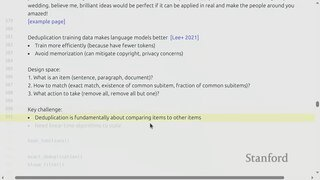
\includegraphics[width=0.92\textwidth]{figures/20_dedup_design.jpg}
\caption{去重设计空间：单元 / 匹配方式 / 动作\protect\footnotemark}
\end{figure}
\footnotetext{视频画面时间区间：00:42:15--00:43:00。}

设计一个去重管线，要回答三个问题：

\begin{enumerate}
    \item \textbf{单元（unit）}是什么？句子、段落、还是整篇文档？
    \item \textbf{如何匹配（match）}？精确匹配，还是基于"共有子项比例"？
    \item \textbf{采取什么动作（action）}？删除所有实例，还是保留一份？
\end{enumerate}

\begin{warningbox}{核心算法挑战}
去重本质上要\textbf{比较项与项之间}的关系——它是\textbf{成对（pair-wise）}的。质量分类是单点的（给一项打分即可），去重却必须两两比较。而这些数据集极其巨大，任何 $O(N^2)$ 的算法都不可行。我们需要某种\textbf{线性时间}的算法，但仍能完成"成对"的判断。
\end{warningbox}

\subsection{基础积木：哈希函数}

\begin{figure}[H]
\centering
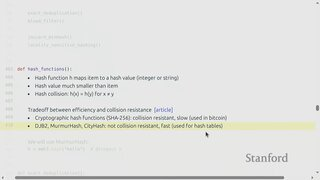
\includegraphics[width=0.92\textwidth]{figures/21_hash_functions.jpg}
\caption{哈希函数回顾：从大对象映射到小整数/字符串\protect\footnotemark}
\end{figure}
\footnotetext{视频画面时间区间：00:44:00--00:44:30。}

哈希函数把一个项（句子、文档）映射到一个比它小得多的哈希值（整数或字符串）。关键性质是可能出现\textbf{哈希冲突}——两个不同项映射到同一个哈希值。在字典/哈希表里冲突通常是坏事，但后面会看到，在控制好的剂量下，冲突反而能为我们所用。

哈希函数有很多种，在\textbf{效率}和\textbf{抗冲突性}之间取舍：加密哈希（如比特币用的）抗冲突但慢；普通哈希表用的哈希不抗冲突但快。我们追求速度，不做加密，所以用 \texttt{murmurhash} 这类快速哈希。

\subsection{精确去重}

\begin{figure}[H]
\centering
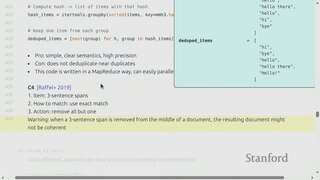
\includegraphics[width=0.92\textwidth]{figures/22_exact_dedup.jpg}
\caption{精确去重：哈希 → 分组 → 每组保留一份\protect\footnotemark}
\end{figure}
\footnotetext{视频画面时间区间：00:46:00--00:46:30。}

最简单的精确去重：项是字符串、要求精确匹配、保留一份。流程是先建一个"哈希值 $\to$ 项列表"的映射，然后每组保留一项。若无哈希冲突，这就是精确去重——"hello" 出现两次就变成一次；"Hello!"（大写加感叹号）则是完全不同的项。

\begin{knowledgebox}{精确去重的优缺点与 C4 实践}
\textbf{优点}：简单、高精度（不会误删你需要的项）、易于 MapReduce 化并行扩展。\par
\textbf{缺点}：无法处理近似重复。\par
C4 就用这个方法：单元是\textbf{三句跨度的 span}，精确匹配，保留一份。讲师吐槽一点：在三句 span 上做"手术"切掉重复段，剩下的文档可能连贯通性都没有，但大家"who cares"就过去了。
\end{knowledgebox}

\subsection{Bloom Filter：内存高效的近似集合}

精确去重的 MapReduce 路线之外，还有一种更"哈希表味儿"的方法：\textbf{Bloom Filter}。它高效、近似、内存友好；可以更新但不能删除；它表示一个集合，查询成员关系时——返回"否"则\textbf{一定不在}，返回"是"则\textbf{大概率在}（有小概率假阳性）。

\subsubsection*{Bloom Filter 的构建与查询}

\begin{figure}[H]
\centering
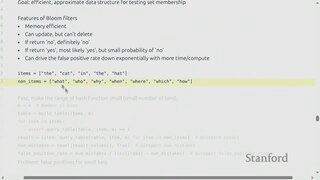
\includegraphics[width=0.92\textwidth]{figures/23_bloom_build.jpg}
\caption{Bloom Filter：位图 + 多个哈希函数；构建时置位，查询时全部命中才算"在"\protect\footnotemark}
\end{figure}
\footnotetext{视频画面时间区间：00:48:00--00:49:30。}

构建步骤：定义 $m$ 个桶（示例里 $m=8$），建一个位数组；对每个项哈希一次，把对应位置 1。"the cat" 哈希到 2，置位第 2 格；"cat" 哈希到 7，置位第 7 格……位数组里\textbf{不保存项本身}，所以你无从知道是否发生了假阳性。查询时，计算待查项的哈希，看对应位是否都为 1。

\begin{warningbox}{单哈希函数的糟糕假阳性率}
用一个哈希函数、$m=8$ 桶时，假阳性率（假阳性数 / 总阳性数）高达 $4/4$，相当糟糕。当然 $m$ 增大会改善——误差概率约为 $1/m$。但若想要误差 $10^{-10}$，桶数会爆炸，内存吃不消。
\end{warningbox}

\subsubsection*{招式：用多个哈希函数}

更聪明的办法是用 $k$ 个哈希函数。每个项被哈希到 $k$ 个（不一定不同的）槽位，全部置 1。查询时只有当 $k$ 个位置\textbf{全部}为 1，才返回"在"。这样假阳性率显著下降。

\subsection{Bloom Filter 的形式化分析}

\begin{figure}[H]
\centering
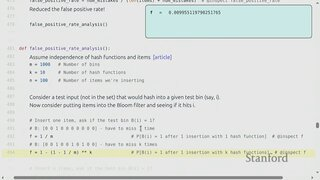
\includegraphics[width=0.95\textwidth]{figures/24_bloom_math.jpg}
\caption{Bloom Filter 假阳性率推导：从单 hash 到 $k$ 个 hash 再到 $n$ 个项\protect\footnotemark}
\end{figure}
\footnotetext{视频画面时间区间：00:54:00--00:57:00。}

设 $m$ 为桶数、$k$ 为哈希函数个数、$n$ 为插入项数。考虑一个\textbf{不在集合中}的测试项，它会被哈希到某个位置 $i$，我们关心"位置 $i$ 是否被置过位"。

\paragraph{第一步：$n=1, k=1$。}只插一个项、只用一个哈希函数。位置 $i$ 被命中的概率就是单次哈希冲突概率：

\[
\Pr[\text{命中 } i] = \frac{1}{m}
\]

\paragraph{第二步：$n=1$，用 $k$ 个哈希函数。}一次"没命中 $i$"的概率是 $1 - 1/m$，$k$ 次都未命中的概率是 $(1-1/m)^k$，所以命中至少一次的概率是 $1 - (1-1/m)^k$。

\paragraph{第三步：插入 $n$ 个项。}位置 $i$ 在 $n \cdot k$ 次独立哈希后仍未被命中的概率为：

\[
\Pr[i \text{ 仍为 } 0] = \left(1 - \frac{1}{m}\right)^{kn}
\]

\paragraph{第四步：测试项的假阳性率。}测试项本身要哈希 $k$ 次，每次都必须命中已置位的位置，所以假阳性率为：

\[
f = \left(1 - \left(1 - \frac{1}{m}\right)^{kn}\right)^k
\]

\begin{importantbox}{最优 $k$ 与渐近行为}
固定 $m/n$ 比例、对 $f$ 求最优 $k$，渐近分析给出 $k^\ast \sim m/n$（哈希函数个数应与"桶数/项数"同阶）。此时位置被置位的概率趋于 $0.5$，假阳性率 $f \approx 0.5^k$。
\par
举例：$m=1000,\ n=100$，则 $k^\ast=10$，$f=0.008$；若取 $k=6$（也接近最优），$f \approx 0.008$。可见适度内存开销就能把假阳性率压到很低。
\end{importantbox}

\begin{practicebox}{Dolma 的实际配置}
Dolma 把假阳性率设为 $10^{-5}$，用 Bloom Filter 做精确去重，去重单元是\textbf{段落}。
\end{practicebox}

\subsection{近似集合成员：Jaccard 相似度}

精确去重抓不到"道德上是重复、但字面有出入"的近似重复。要处理近似重复，需要一个\textbf{相似度度量}。最常用的是 \textbf{Jaccard 相似度}：

\[
J(A, B) = \frac{|A \cap B|}{|A \cup B|}
\]

例：$A=\{1,2,3,4\},\ B=\{1,2,3,5\}$，交集大小为 3、并集大小为 5，故 $J=3/5=0.6$。

\begin{figure}[H]
\centering
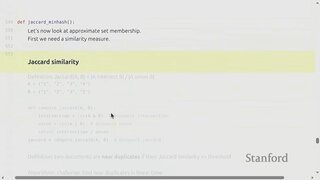
\includegraphics[width=0.92\textwidth]{figures/25_jaccard.jpg}
\caption{Jaccard 相似度：交集除以并集\protect\footnotemark}
\end{figure}
\footnotetext{视频画面时间区间：00:59:00--00:59:40。}

我们说"两个文档是近似重复"当且仅当它们的 Jaccard 相似度超过某阈值（一般很高，比如 0.9，意味着只差一个逗号那种）。注意 Jaccard \textbf{没有语义}——你完全可能把 "not" 这个词漏掉、含义彻底反转，但 Jaccard 仍很高。它只关心字面是否近似。

\begin{warningbox}{算法挑战重申}
如何在线性时间内找出近似重复？Jaccard 是成对函数——只能对两个元素算。我们要想办法把它改写成\textbf{只依赖单个元素}的哈希函数。
\end{warningbox}

\subsection{MinHash：把 Jaccard 变成一元函数}

\textbf{MinHash} 就是这样一个哈希函数，它有一个绝妙性质：\textbf{两个集合的 MinHash 发生冲突的概率，恰好等于它们的 Jaccard 相似度}。

\begin{figure}[H]
\centering
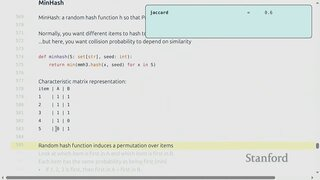
\includegraphics[width=0.92\textwidth]{figures/26_minhash.jpg}
\caption{MinHash：对集合中所有元素哈希后取最小值；冲突概率 = Jaccard\protect\footnotemark}
\end{figure}
\footnotetext{视频画面时间区间：00:62:00--00:64:00。}

定义：对一个集合 $S$，把其中所有元素用某个随机哈希函数哈希，取\textbf{最小值}作为 MinHash：

\[
\mathrm{minhash}(S) = \min_{x \in S} h(x)
\]

初看并不显然"取个 min"就能让期望等于 Jaccard，但论证其实很简单。考虑集合 $A,B$，把它们的元素排成一个\textbf{指示矩阵}（行是所有可能元素，列是 $A$、$B$，标记某元素是否在集合中）。随机哈希函数相当于在这些行上诱导一个\textbf{随机排列}。

\begin{knowledgebox}{为什么 MinHash 冲突概率等于 Jaccard？}
随机排列下，每一行（每个元素）成为"第一个"的概率相等。看 $A$ 和 $B$ 各自的第一个（即最小哈希对应的）元素：
\begin{itemize}
    \item 若"第一个"落在 $A \cap B$（交集）中——比如元素 $1,2,3$——那么 $A$ 和 $B$ 的 MinHash 都等于这个元素的哈希值，\textbf{冲突}。
    \item 若"第一个"落在 $A \setminus B$ 或 $B \setminus A$（比如 4 或 5），则 $A$ 的第一个与 $B$ 的第一个不同，\textbf{不冲突}。
\end{itemize}
因此冲突概率恰好等于"第一个落在交集中"的概率，即 $|A \cap B| / |A \cup B| = J(A,B)$。
\end{knowledgebox}

讲师用 1000 次随机哈希做实验，估计出的 Jaccard 约为 0.6（有少量舍入误差），与真值吻合。

\begin{importantbox}{但还差一步}
现在我们把成对的 Jaccard 简化成了一元哈希函数——但仅仅"冲突"并不能告诉我们两个集合相似。冲突只是\textbf{更可能发生在相似集合之间}。我们想要更强的保证：Jaccard 超过阈值就几乎必冲突，低于阈值就几乎必不冲突。
\end{importantbox}

\subsection{Locality Sensitive Hashing：锐化阈值}

\begin{figure}[H]
\centering
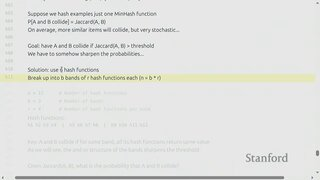
\includegraphics[width=0.92\textwidth]{figures/27_lsh_bands.jpg}
\caption{LSH：把 $n$ 个 MinHash 分成 $b$ 个 band、每 band $r$ 个；某 band 全相同则冲突\protect\footnotemark}
\end{figure}
\footnotetext{视频画面时间区间：00:66:00--00:67:30。}

\textbf{Locality Sensitive Hashing（LSH）}的招式还是"用更多哈希函数"，但这次有结构：把 $n$ 个哈希函数分成 $b$ 个\textbf{band}，每 band 含 $r$ 个哈希函数（如 $n=12,\ b=3,\ r=4$）。判定 $A,B$ 冲突的条件是：\textbf{至少存在一个 band，其 $r$ 个哈希值全部相同}。这是一种"或-与"（OR of AND）结构，是锐化阈值的关键。

\subsubsection*{碰撞概率推导}

设 $\mathrm{sim} = J(A,B)$。单个哈希函数冲突的概率是 $\mathrm{sim}$。

\begin{itemize}
    \item \textbf{固定一个 band 全部匹配的概率}：$\mathrm{sim}^r$（$r$ 个哈希全部相同）。
    \item \textbf{固定一个 band 不匹配的概率}：$1 - \mathrm{sim}^r$。
    \item \textbf{所有 $b$ 个 band 都不匹配的概率}：$(1 - \mathrm{sim}^r)^b$。
    \item \textbf{至少一个 band 匹配（即冲突）的概率}：
\end{itemize}

\[
P(\text{collision}) = 1 - \left(1 - \mathrm{sim}^r\right)^b
\]

\begin{importantbox}{一个具体算例}
$\mathrm{sim}=0.8$、$b=5$ 个 band、每 band $r=10$ 个哈希（共 50 个哈希）：
\begin{itemize}
    \item 固定 band 匹配概率：$0.8^{10} \approx 0.107$。
    \item 全部 5 个 band 都不匹配的概率：$(1-0.107)^5 \approx 0.563$。
    \item 至少一个 band 匹配（冲突）的概率：$1 - 0.563 \approx 0.437$。
\end{itemize}
对比单哈希时直接是 $0.8$——曲线被"重塑"了。
\end{importantbox}

\subsubsection*{S 曲线：调 $b$、$r$ 塑造阈值}

你头脑里应有的图景是：横轴为相似度 $\mathrm{sim}$，纵轴为冲突概率，希望曲线在阈值附近\textbf{陡峭跃迁}（像 sigmoid）。阈值以下几乎为 0、以上几乎为 1。

\begin{figure}[H]
\centering
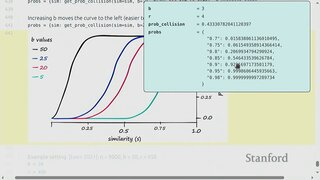
\includegraphics[width=0.92\textwidth]{figures/28_lsh_sigmoid.jpg}
\caption{LSH S 曲线：增大 $r$ 右移并锐化，增大 $b$ 左移\protect\footnotemark}
\end{figure}
\footnotetext{视频画面时间区间：00:71:00--00:73:00。}

\begin{itemize}
    \item \textbf{增大 $r$}（每 band 哈希数）：曲线\textbf{右移}（更难匹配）并\textbf{锐化}。例如把 $r$ 从 10 提到 20：原本 $\mathrm{sim}=0.7$ 时冲突概率 0.24 太高，提到 $r=20$ 后降到 0.07 左右。
    \item \textbf{增大 $b$}（band 数）：曲线\textbf{左移}。原来 $\mathrm{sim}=0.9$ 时冲突概率不够高，增大 $b$ 后可以推到 90 以上。
\end{itemize}

通过恰当设置 $b$ 和 $r$，能得到非常锐利的 sigmoid。

\begin{knowledgebox}{阈值处的极限与一个真实案例}
\textbf{极限}：在阈值处，碰撞概率收敛到 $1 - 1/e \approx 0.632$。\par
\textbf{真实案例}：某论文（上一讲见过）用 MinHash LSH 做近似去重，取 $b=20$、$r=450$。$r$ 很大意味着想要极锐利的阈值。由公式可算出阈值约为 $0.99$——即每 100 个词只允许差 1 个词，相当严格。在阈值处，固定 band 匹配概率 $0.99^{450} \approx 0.05$，整体碰撞概率 $\approx 0.64$（与 $1-1/e$ 吻合）。一旦相似度高于阈值，几乎必冲突；低于阈值，几乎必不冲突。
\end{knowledgebox}

\subsection{去重课堂问答}

\paragraph{问：合成数据（synthetic data）越来越多，如何对"改写敏感"地去做重？}
答：有一些论文（如 SemDeDup，本讲未展开）用\textbf{嵌入（embedding）}做更语义化的相似度。这套思路完全契合 LSH 框架——LSH 本就是为近似最近邻设计的。你只要把文档嵌入到一个向量空间，就能在该空间找最近邻。代价是跑嵌入更贵，而且我们目前主要处理"非常近的近似重复"。若做得太模糊，可能会误删大量数据，要非常小心。

\paragraph{问：高质量数据是否反而"想要"重复？}
答：对。在语言建模里有一个\textbf{mid-training} 阶段，你确实想对高质量数据多跑几个 epoch。所以去重更适用于\textbf{预训练}——清洗掉那 61,000 份随机副本。最优做法未必是"全部删到只剩一份"：可以记录一份文档出现的次数，用次数的平方根或对数作为权重，让它\textbf{不是等比例}出现、但仍被承认"重要到值得多过几遍"。

\section{总结}

\begin{figure}[H]
\centering
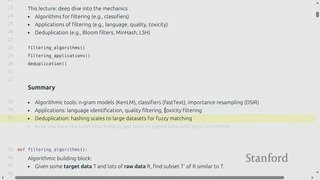
\includegraphics[width=0.92\textwidth]{figures/29_summary.jpg}
\caption{本讲总结：过滤 + 去重两套算法工具箱\protect\footnotemark}
\end{figure}
\footnotetext{视频画面时间区间：00:78:00--00:79:05。}

\begin{importantbox}{两大工具箱回顾}
\textbf{过滤}：n-gram 模型、线性分类器、重要性重采样。凡是有目标数据集、想获取更多同分布数据，都能套这套工具。若没有目标数据集但有强语言模型，可以让它合成或筛出 $T$，再训一个快分类器。可用于语言识别、质量过滤、毒性过滤等。
\par\medskip
\textbf{去重}：减少算力浪费、避免记忆。算法积木是\textbf{哈希}——它把成对的相似度/冲突概念转化为一元函数，从而具备线性时间性质。精确去重用哈希表或 Bloom Filter；近似去重用 MinHash + LSH。我们看到了用多哈希函数 + "与/或"结构（LSH 的 band）来塑造判定曲线的精巧方法。
\end{importantbox}

\begin{practicebox}{ Assignment 4 的衔接}
关于"如何教数据"，本讲只是开始。真正的直觉来自\textbf{亲自花时间看数据、过滤、训练模型}——这正是 Assignment 4 要让你做的事。下一讲起将进入课程最后一个单元：强化学习与对齐（alignment）。
\end{practicebox}

\end{document}
